\documentclass[12pt, a4paper]{article}
\usepackage[russian]{babel}
\usepackage{fontspec}
\setsansfont{Calibri}
\setmonofont{Consolas}
\setmainfont[
    Ligatures=TeX,
    Extension=.otf,
    BoldFont=cmunbx,
    ItalicFont=cmunti,
    BoldItalicFont=cmunbi,
]{cmunrm}
\usepackage{polyglossia}
\setdefaultlanguage{russian}
\setotherlanguage{english}


\usepackage{geometry}
\usepackage{pgfplotstable}

\geometry{
margin=2cm
}


\usepackage{indentfirst}

\usepackage{arydshln}
\usepackage[fleqn]{amsmath}
\usepackage{xfrac}
\usepackage{esint}
\usepackage{amssymb}
\usepackage{mathbbol}
\usepackage[T1]{fontenc}
\usepackage{mathtools}
\usepackage{color}
\usepackage{ulem}
\usepackage{tabu}
\usepackage{multicol}
\usepackage{multirow}
\usepackage{rotating}

\usepackage[outline]{contour}
\contourlength{1.2pt}

%\usepackage{tikz}
\usepackage{graphics}
\usepackage{xcolor}

\usepackage{pgfplots}
\usepackage{pgfplotstable}


\usepackage[at]{easylist}

\DeclareMathOperator{\sign}{sign}

%-------------------------------------------------------------------------------
%-------------------------------------------------------------------------------
%-------------------------------------------------------------------------------


\newcommand{\insertTitle}[7]{
\begin{titlepage}
	\begin{center}
    	\large
		Министерство науки и высшего образования Российской Федерации
		
		Новосибирский государственный технический университет
		%\vspace{0.25cm}
		\vfill
		{\textbf #1}
		
		Лабораторная работа №#2
		\vfill
	\end{center}
	
	\begin{tabular}{ m{7em}  m{7em} }
	Факультет: & ФПМИ \\ 
	Группа: & #3 \\  
	Студенты: & #4 \\
	& #5 \\
	Вариант: & #6
	\end{tabular}
	\vfill

\begin{center}
Новосибирск

#7
\end{center}
\end{titlepage}
}


\pgfplotstableset{
%\rowcolors{2}{gray!25}{white}
	begin table={\begin{tabular}},
	end table=\end{tabular},
}




\usepackage{slashbox}
\newcommand{\inputTableOne}[1]{
\begin{center}
\noindent\pgfplotstabletypeset[
	columns={a, $1$, $5e-1$, $1e-1$, $5e-2$, $1e-2$},
	columns/a/.style={string type, column name={\backslashbox{$P$}{$\varepsilon$}}},
	columns/$0.1$/.style={string type, column name={$0.1$}},
	columns/$0.3$/.style={string type, column name={$0.3$}},
	columns/$0.5$/.style={string type, column name={$0.5$}},
	columns/$0.7$/.style={string type, column name={$0.7$}},
	columns/$0.9$/.style={string type, column name={$0.9$}},
	every head row/.style={before row=\hline,after row=\hline\hline}, 
	every last row/.style={after row=\hline},
	column type/.add={|}{|},
	col sep=tab,
]{#1}
\end{center}
}


\newcommand{\inputTableTwo}[1]{
\begin{center}
\noindent\pgfplotstabletypeset[
	columns={a, $алгоритм1$, $алгоритм2$, $алгоритм3$ },
	columns/a/.style={string type, column name={\backslashbox{m}{алгоритм}}},
	columns/$алгоритм1$/.style={string type, column name={$\text{алгоритм 1}$}},
	columns/$алгоритм2$/.style={string type, column name={$\text{алгоритм 2}$}},
	columns/$алгоритм3$/.style={string type, column name={$\text{алгоритм 3}$}},
	every head row/.style={before row=\hline,after row=\hline\hline}, 
	every last row/.style={after row=\hline},
	column type/.add={|}{|},
	col sep=tab,
]{#1}
\end{center}
}



\usepackage[utf8]{inputenc}
\usepackage{listings}
\usepackage{color}
 
\definecolor{codegreen}{rgb}{0,0.6,0}
\definecolor{codegray}{rgb}{0.5,0.5,0.5}
\definecolor{codepurple}{rgb}{0.58,0,0.82}
\definecolor{backcolour}{rgb}{0.85,0.85,0.85}
 
\lstdefinestyle{mystyle}{
	backgroundcolor=\color{backcolour},   
	commentstyle=\color{codegreen},
	keywordstyle=\color{blue},
	basicstyle=\fontsize{10}{12}\selectfont\ttfamily,
   	numberstyle=\tiny\color{codegray},
	stringstyle=\color{codepurple},
    	breakatwhitespace=false,         
	breaklines=true,                 
	captionpos=b,                    
	keepspaces=true,                 
	numbers=left,                    
	numbersep=5pt,                  
	showspaces=false,                
	showstringspaces=false,
	showtabs=false,                  
	tabsize=4
}
\lstset{ style=mystyle}



\newcommand{\myCodeInput}[3]{
{\bf #2}
\lstinputlisting[language=#1]{#3}
}

% Размер изображений [0, 1]
\newcommand{\picSize}{0.7}

\setlength{\abovedisplayskip}{-1pt}
\setlength{\belowdisplayskip}{-1pt}


\usepackage{subfig}
\newcommand{\inputTwoImages}[2]{
\begin{figure}[htbp!]
    \noindent
        \includegraphics[width=0.48\textwidth]{#1}
        \includegraphics[width=0.48\textwidth]{#2}
\end{figure}

}




%-------------------------------------------------------------------------------
%-------------------------------------------------------------------------------
%-------------------------------------------------------------------------------


\begin{document}

%-------------------------------------------------------------------------------
%-------------------------------------------------------------------------------
%-------------------------------------------------------------------------------
\insertTitle{Методы оптимизации}{4}{ПМ-63}{Кожекин М.В.}{Утюганов Д.С.}{5}{2019}




%-------------------------------------------------------------------------------
%-------------------------------------------------------------------------------
%-------------------------------------------------------------------------------
\section{Цель работы}

Ознакомиться со статистическими методами поиска при решении задач нелинейного программирования. Изучить методы случайного поиска при определении глобального экстремума функции.




%-------------------------------------------------------------------------------
%-------------------------------------------------------------------------------
%-------------------------------------------------------------------------------
\section{Задание}

1. Реализовать программу для решения задачи поиска глобального экстремума с использованием метода {\bf простого случайного поиска, 1-3 алгоритмов глобального поиска}.

2. Исследовать метод простого случайного поиска при различных $\varepsilon$ и P

\begin{tabular}{ | l | l | l | l | l |}
	\hline
		$\varepsilon$ & P & N & (x, y) & f(x, y) \\ \hline
		 &  &  &  & \\
	\hline
\end{tabular}



3. Провести сравнительный анализ 1-3 алгоритмов глобального поиска по точности получаемого решения и числу вычислений целевой функции. Исследование провести при различных значениях числа попыток  .


Условие задачи:

Найти {\bf максимум} заданной функции:

\[ f(x,y)=  \sum_{i=1}^{6} \frac{C_i}{1 + (x-a_i)^2 + (y - b_i)^2}\]

по области $-10 \leq x \leq 10, -10 \leq y \leq 10$

{\bf Вариант 5}


\begin{tabular}{ | l | l | l | l | l | l | l |}
	\hline
		$i$ & 1 & 2 & 3 & 4 & 5 & 6\\ \hline
		$C_i$ & 1 & 2 & 10 & 5 & 7 & 9 \\ \hline
		$a_i$ & 0 & 0	 & 3 & -7 & 6 & 6 \\ \hline
		$b_i$ & -1 & -4 & -2 & -6 & -10 & 1 \\
	\hline
\end{tabular}

Изобразим целевую функцию:

\begin{multicols}{2}
    \hfill
    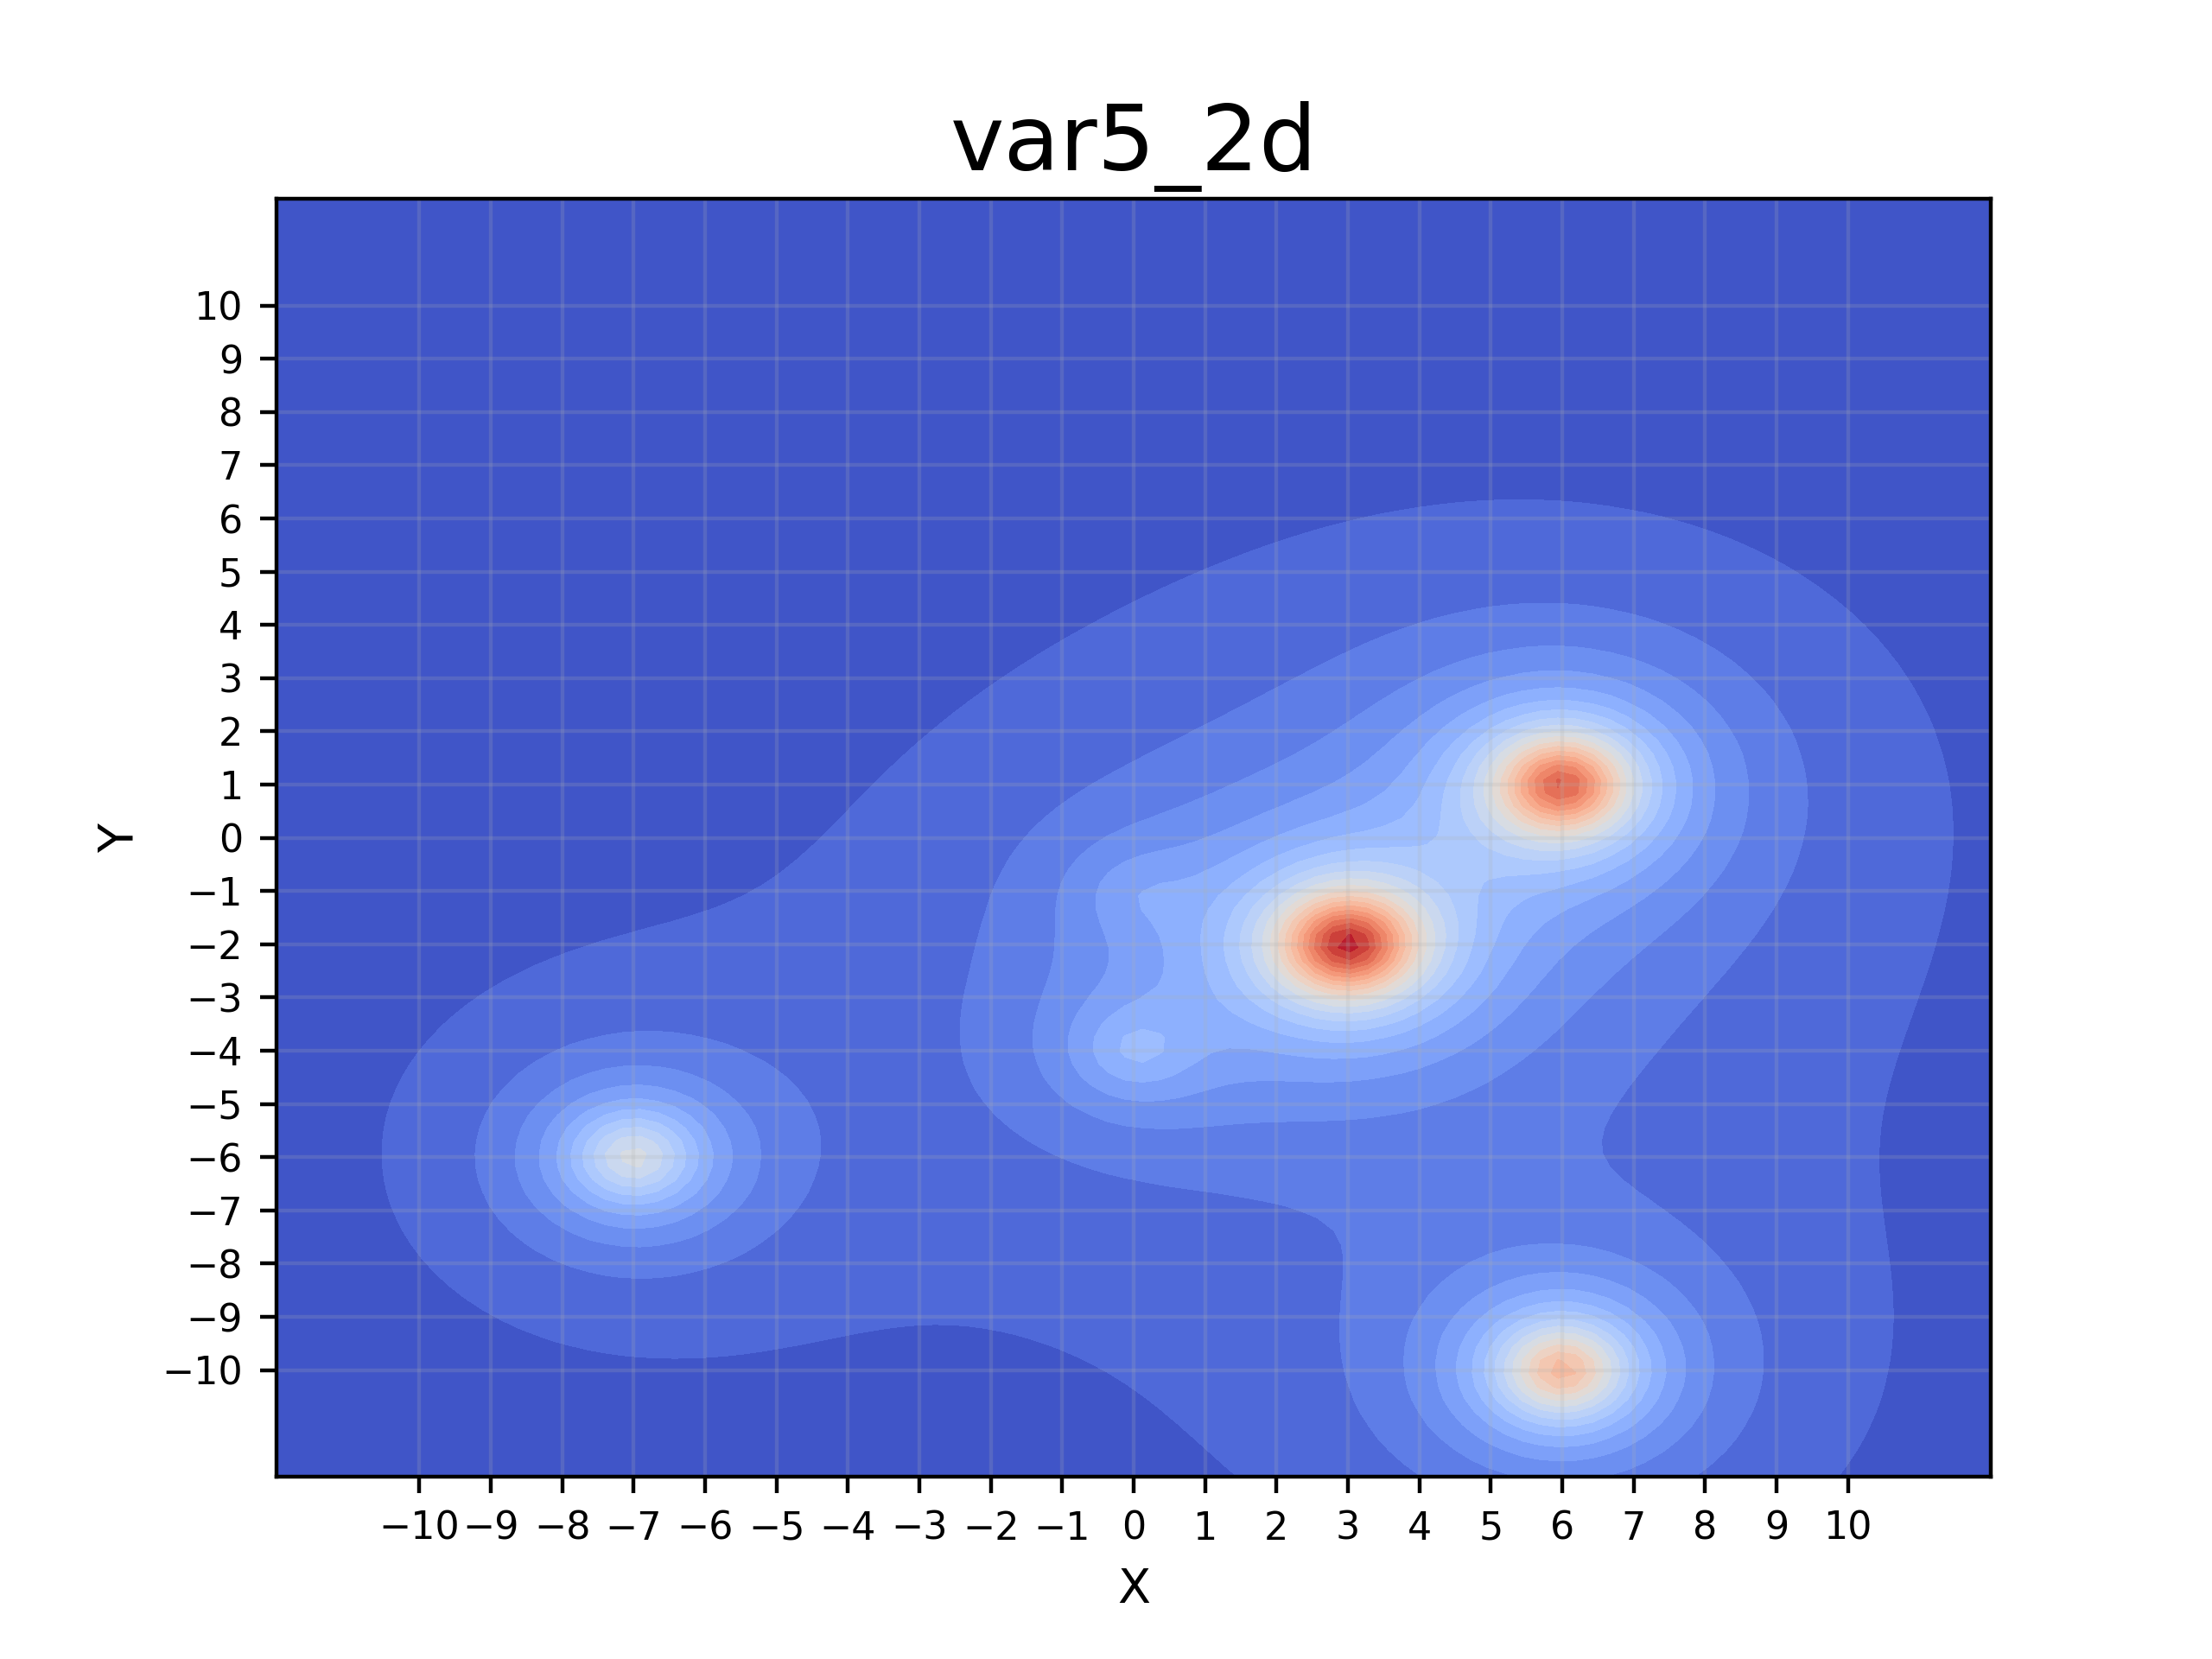
\includegraphics[width=\linewidth]{../pics/var5_2d.png}
    \hfill
    \label{figLeft}
    \hfill
    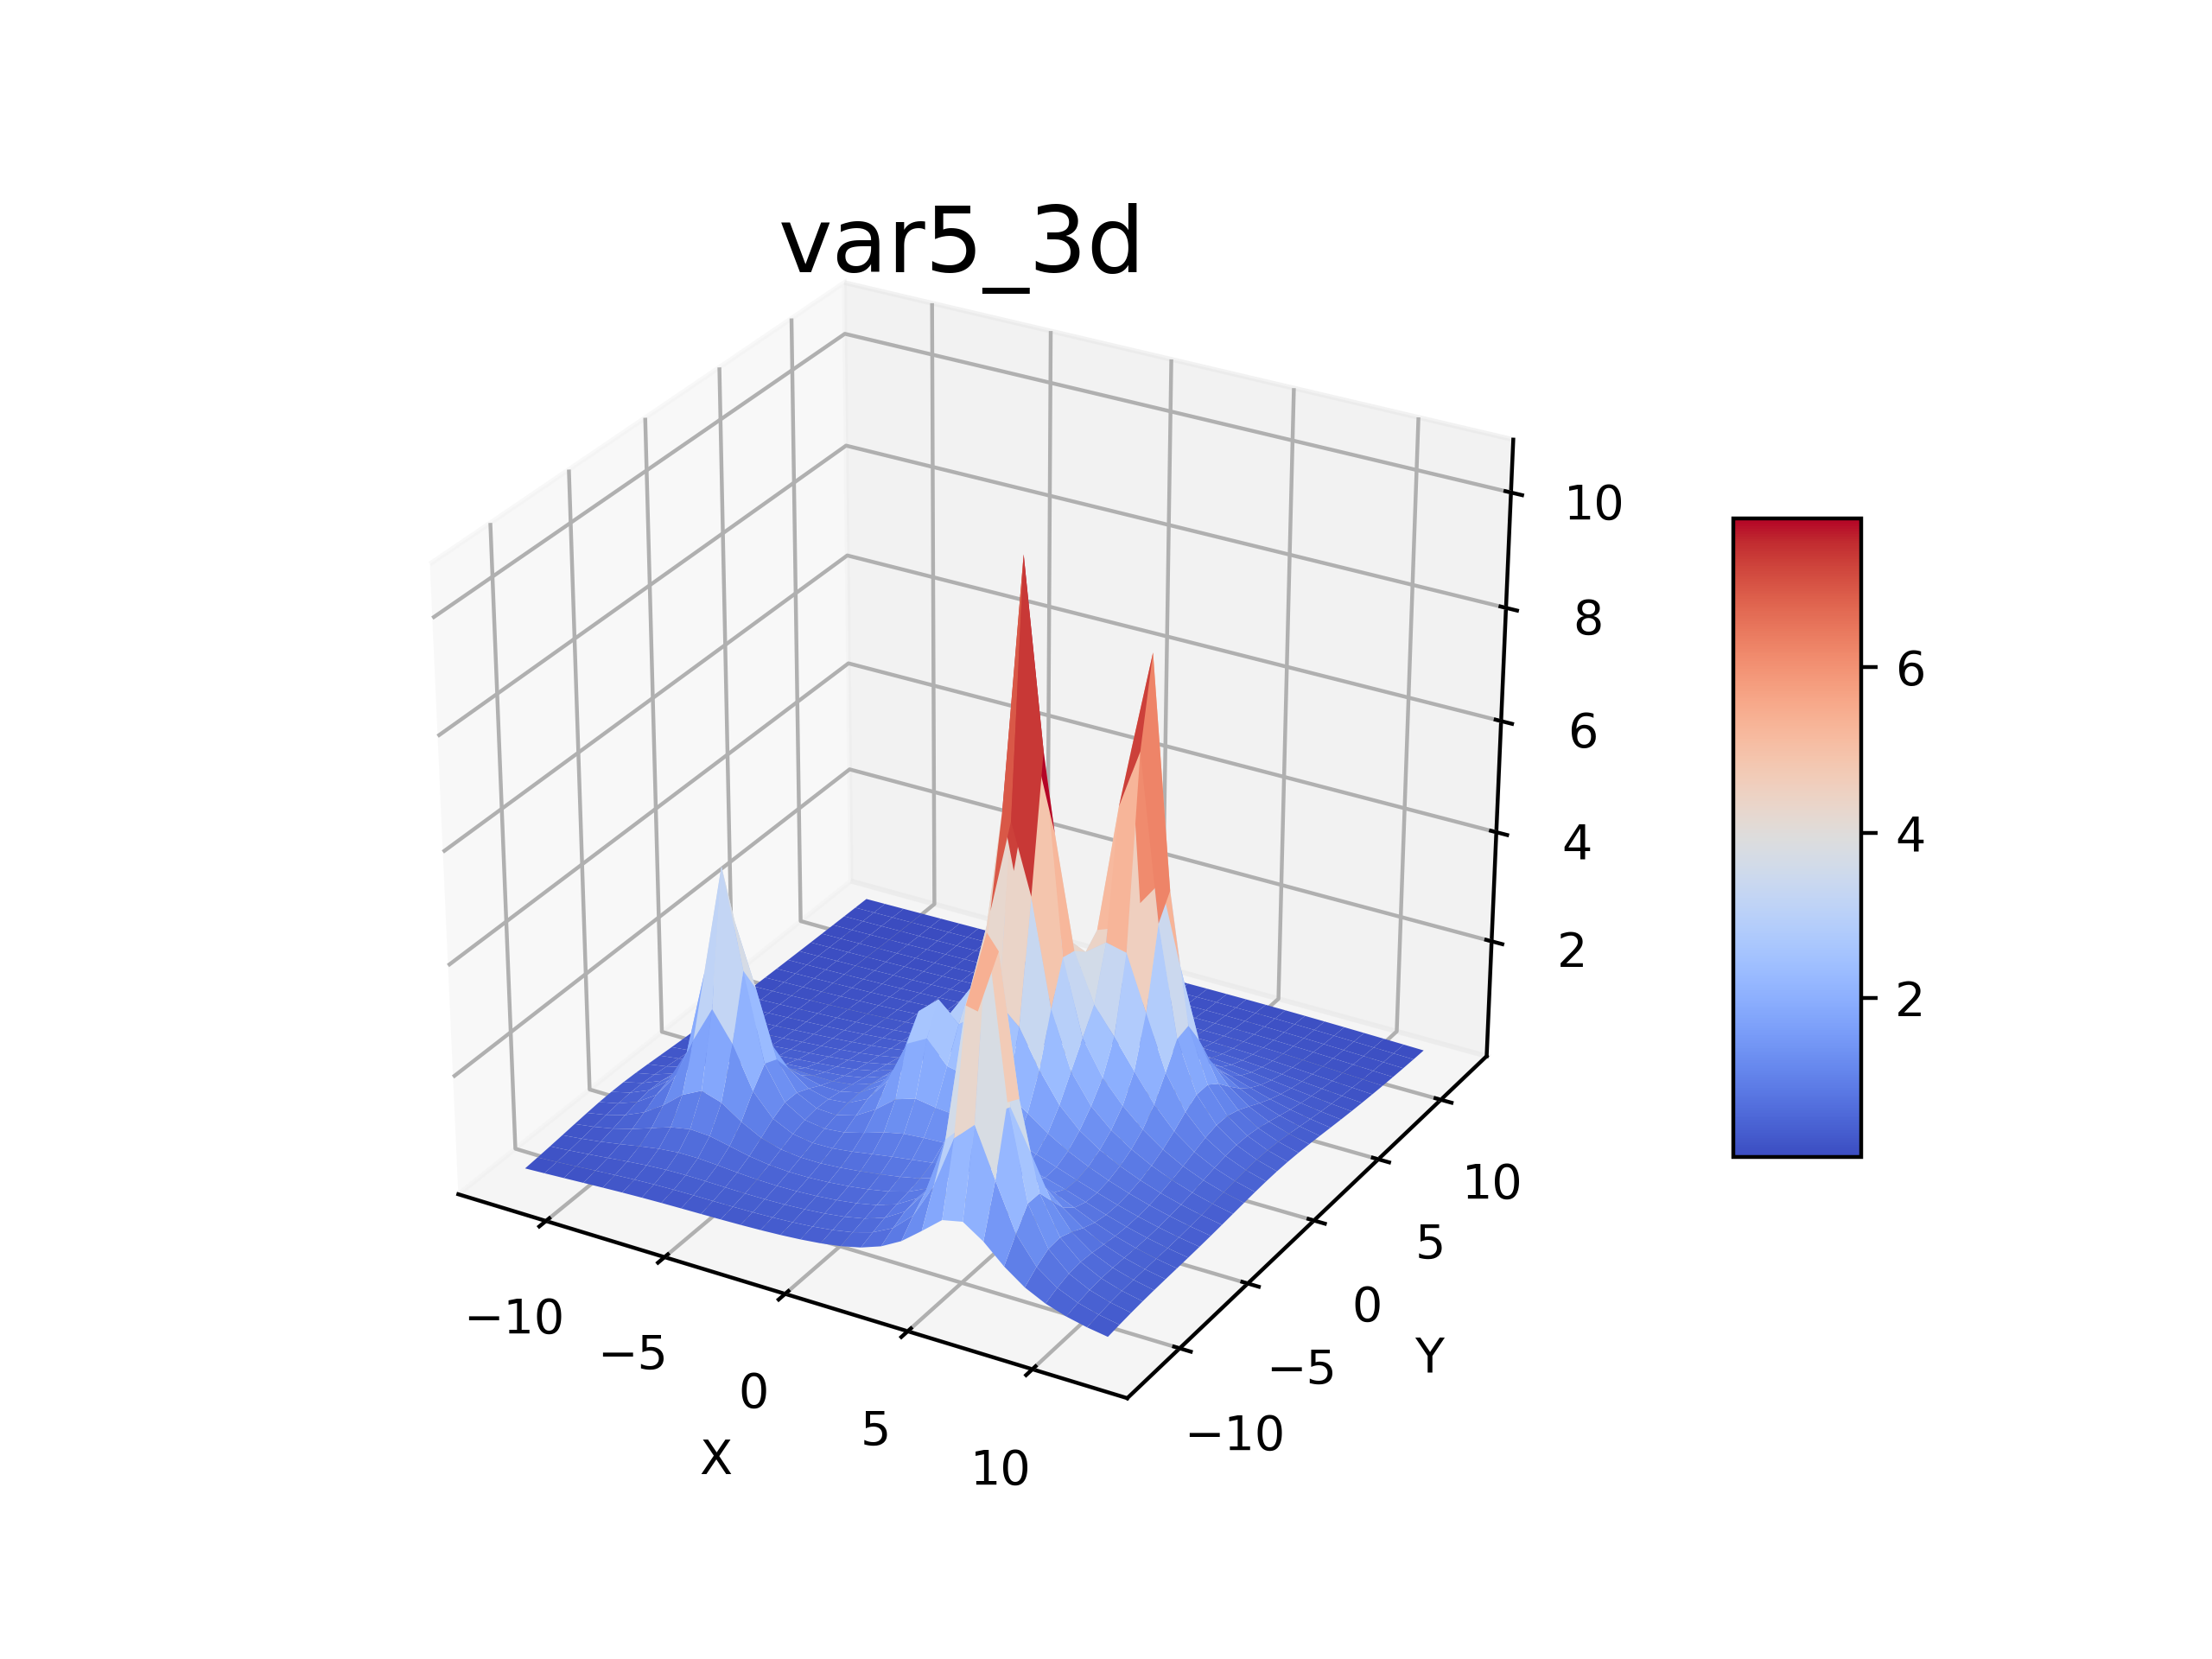
\includegraphics[width=\linewidth]{../pics/var5_3d.png}
    \label{figRight}
\end{multicols}


Кажется, что её максимум это точка (3, -2), но программа находит истинный супремум: 

\begin{figure}
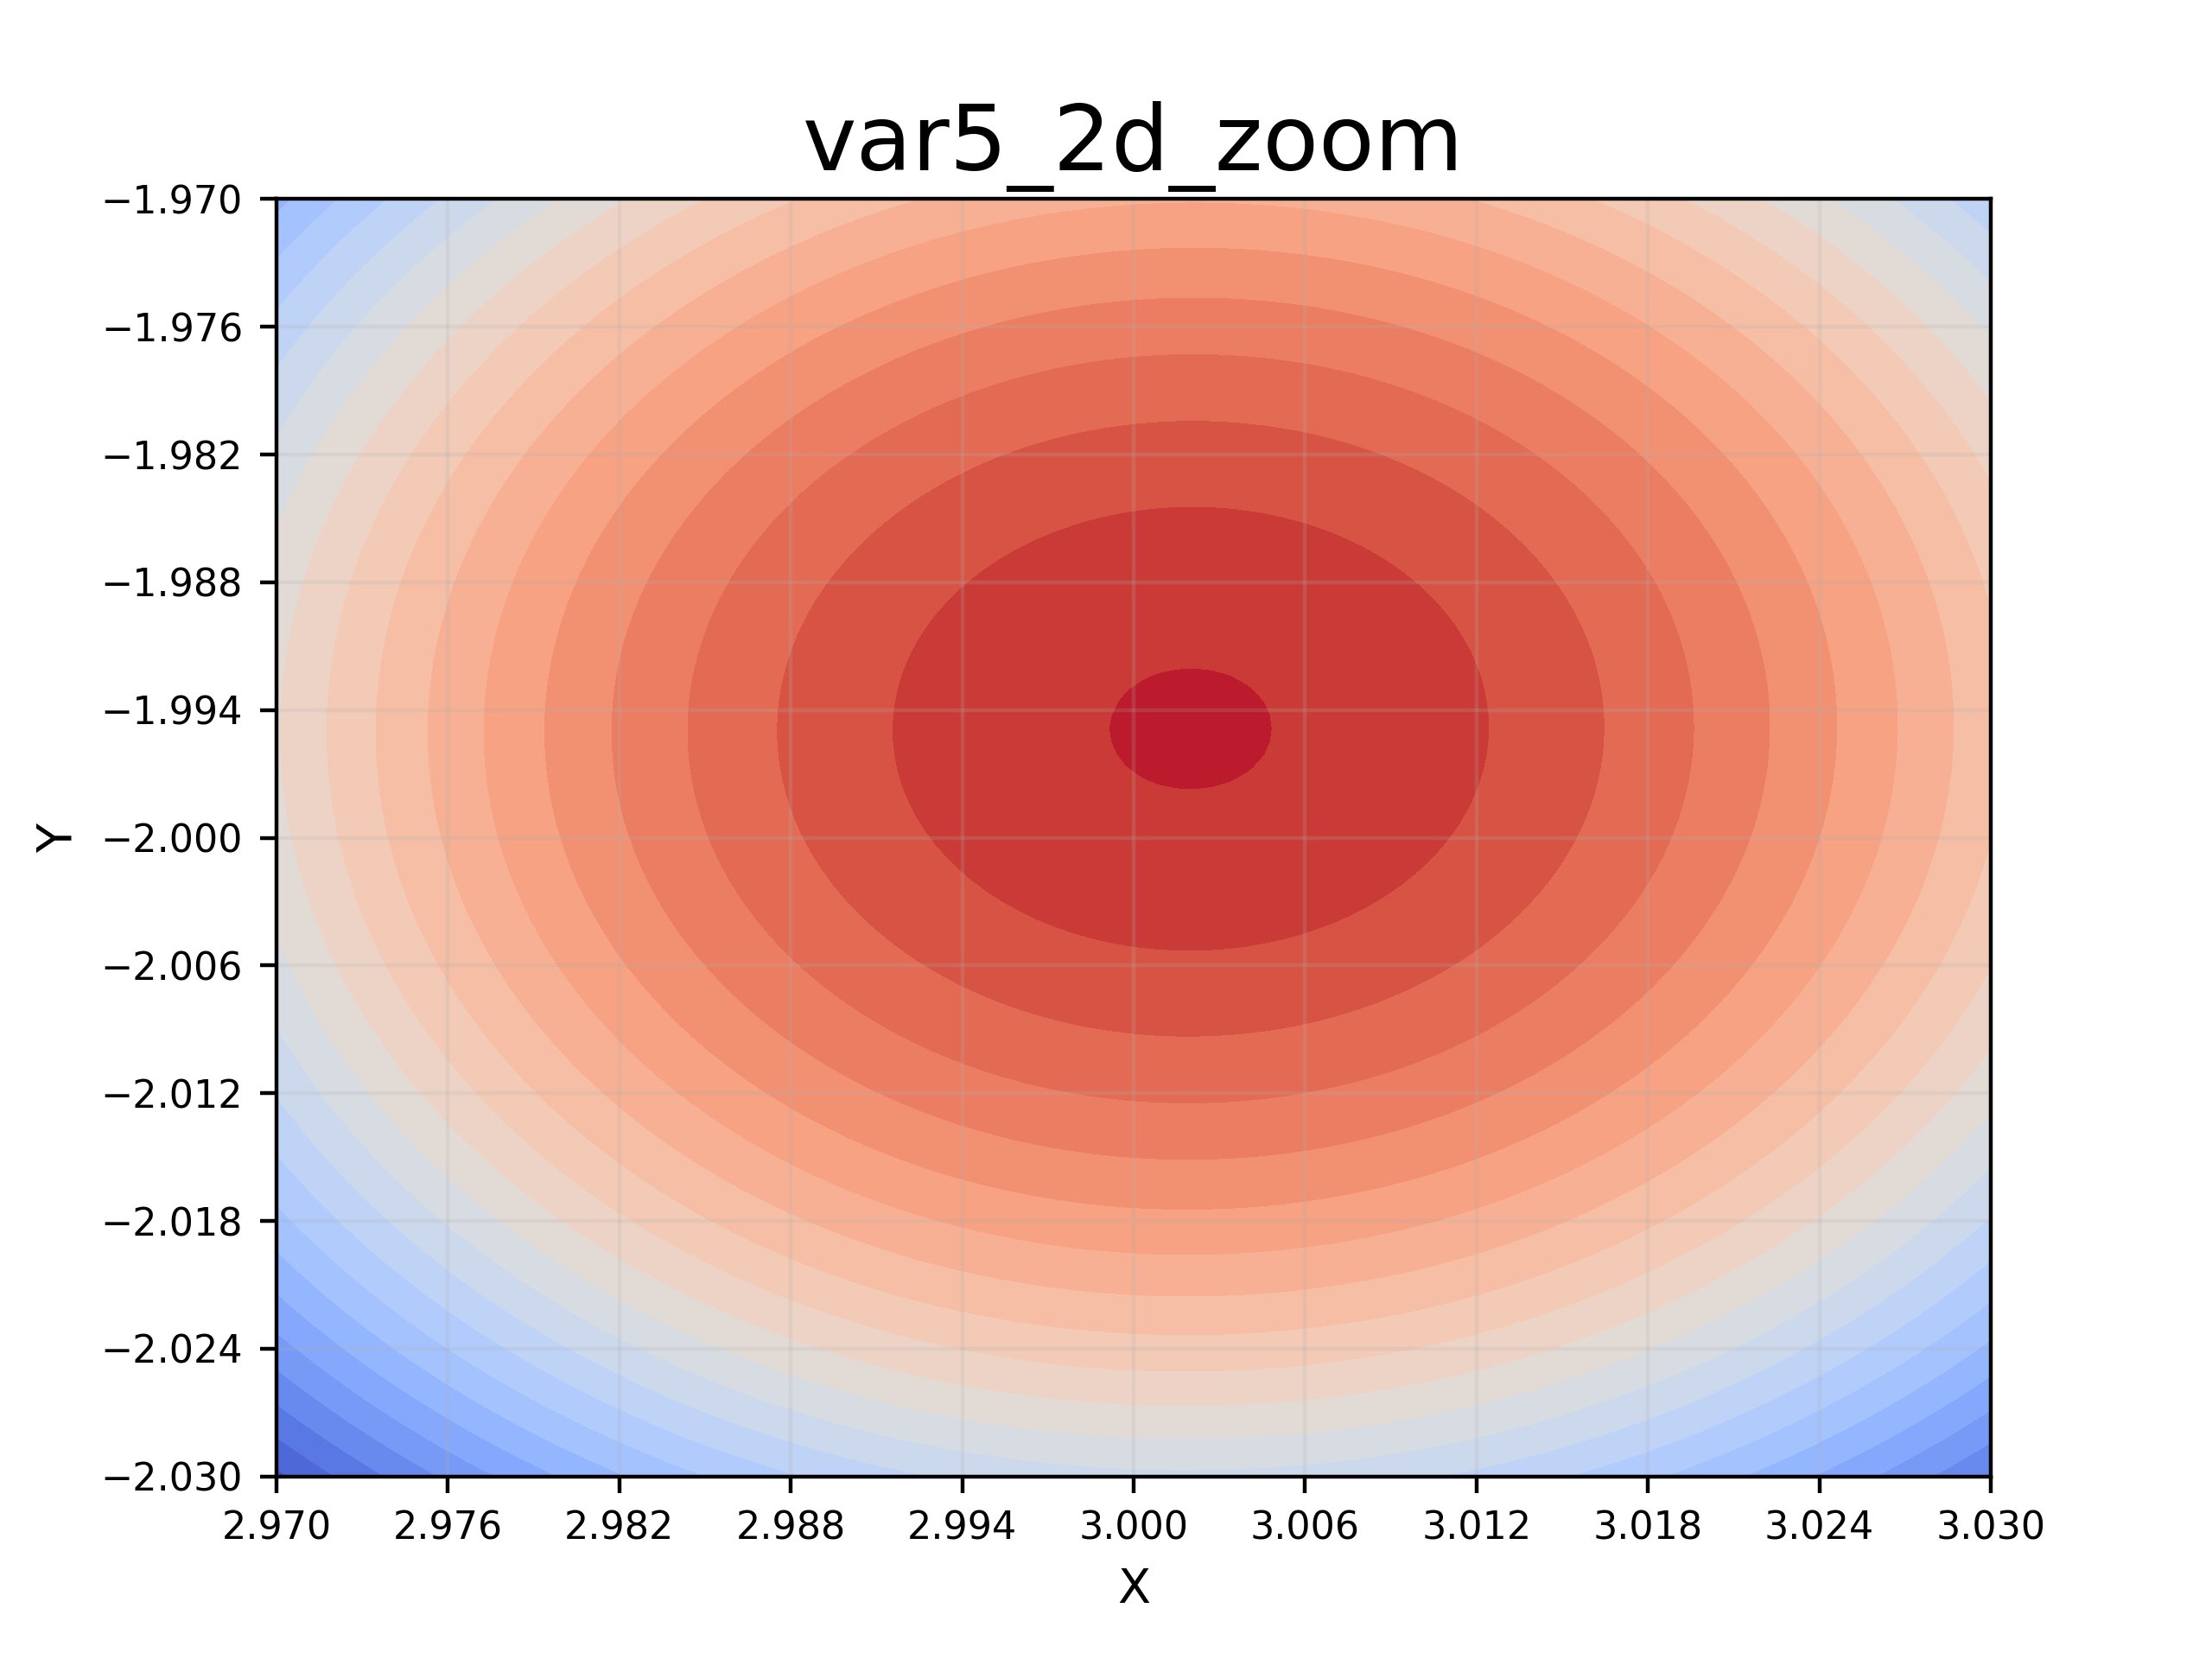
\includegraphics[width=\linewidth]{../pics/var5_2d_zoom.png}
\end{figure}


%-------------------------------------------------------------------------------
%-------------------------------------------------------------------------------
%-------------------------------------------------------------------------------
\section{Зависимость скорости сходимости метода простого случайного поиска при различных $\varepsilon$ и P}
\inputTableOne{table1.txt}
%-------------------------------------------------------------------------------
\subsection{Вывод}
С ростом точности или вероятности растёт и число попыток, необходимых для поиска глобального максимума.



%-------------------------------------------------------------------------------
%-------------------------------------------------------------------------------
%-------------------------------------------------------------------------------
\section{Сравнительный анализ 1-3 алгоритмов глобального поиска по точности получаемого решения и числу вычислений целевой функции}
\inputTableTwo{table2.txt}
%-------------------------------------------------------------------------------
\subsection{Вывод}
Исходя из результатов мы можем заметить, что второй алгоритм считает быстрее всех.
Это обусловлено тем, что мы не запускаем детерминированный алгоритм поиска из тех точек, которые не дадут нам лучшего решения.

С ростом числа точек m мы замечаем рост точности решения и рост числа вычислений целевой функции.





%-------------------------------------------------------------------------------
%-------------------------------------------------------------------------------
%-------------------------------------------------------------------------------
\section{Исходный код программы}
\myCodeInput{c++}{head.h}{../head.h}
\myCodeInput{c++}{main.cpp}{../main.cpp}
\myCodeInput{python}{plot.py}{../plot.py}

\end{document}